\scanpage{3}
\mspage{(1)}
Complexe DR à p.d. et ombres des modules.

\margin{Plan conf. IHES en 1976\figure{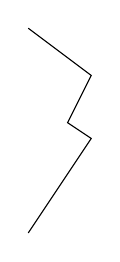
\begin{tikzpicture}\draw (0,2.6)--(.8,2)--(.5,1.4)--(.8,1.2)--(0,0);\end{tikzpicture}}}
\margin{géom. diff.\\ -- anal.\\ -- algébr.\\ \deleted{\unsure{top.}} arithm.\\ top. alg. $\left\{\begin{array}{l}\mathrm{PL}\\ \unsure{\frac12\text{ simpl.}}\end{array}\right.$}

1 Historique

a) Notion des formes diff. (\uline{Poincaré} ?) et formule de \uline{Stokes}
\[
\int_c d\omega=\int_{\partial c}\omega
\qquad(\text{d'où }H^*_{\mathrm{DR}}(X)\longrightarrow H^*(X,\mathbb C))
\]

b) Th. de \uline{De Rham} (conjecturé par \uline{E. Cartan}). \unsure{Mais démonstr.}
\inserted{Maintenant bien compris : th. des faisceaux, lemme Poincaré}

c) Théorie de \uline{Hodge des} intégrales harmoniques
(structure supplémentaire bigraduée sur $H^*_{\mathrm{DR}}(X)$ si $X$ kählérienne compacte)

d) Théorème de \uline{Cartan-Serre} sur variétés de Stein
(ou Lemme de Poincaré valable dans l'analytique \uline{complexe})

e) Cas des variétés algébriques \unsure{ou} schémas, sur corps \unsure{(ou schém. de base finis ?)} : \uline{Dwork}, \uline{Washnitzer} -- \uline{Monsky}, plus tard le yoga ``cristallin'' développé par \uline{Berthelot}, \uline{Illusie}, \deleted{\unsure{et différents}} \inserted{\uline{Messing}, Mazur} \deleted{\unsure{autres}}. \margin{avec Hartshorne, Herrera, Ogus, Bloch (!)} Ici on trouve des théories coh. qui ne sont plus à ``anneau de coeff'' de car. nulle i.e. contenant $\mathbb Q$ -- \unsure{i.e.} en principe les phénomènes de torsion ne sont pas perdus.
\inserted{Du pt de vue Weil, c'était un défaut impardonnable !}

f) Th. de \uline{Grothendieck} pour variétés algébriques sur $\mathbb C$ (\deleted{\unsure{généralisé}} \inserted{\uline{généralisé}} par \uline{Deligne}, \uline{Hartshorne} pour des coeff plus généraux) Ceci donne \unsure{un sens} (au moins en car. 0) à la \uline{signification} topologique de la coh. de De Rham ``\uline{algébrique}'' des schémas algébriques.

g) Complexe de De-Rham-Sullivan pour espaces topologiques généraux : \uline{formes différentielles singulières} $C^\infty$ \deleted{\unsure{\mathbb C}\unsure{-alg. resp.}} $\mathbb C$-algébrique, resp. $\mathbb R$-algébrique resp. $\mathbb Q$-algébrique). Donne la coh. à coeff dans $\mathbb C$ (resp. $\mathbb R$, resp. $\mathbb Q$) (facile). Sullivan montre même

\margin{\diagram{\begin{tikzcd}
C^\bullet_{\mathrm{DRS}\,\mathbb R\text{-alg}} \arrow[r,phantom,"\unsure{\subset}" description] & C^\bullet_{\mathrm{DRS}\,C^\infty} \arrow[r,phantom,"\subset" description] \arrow[d,phantom,"\cup" description] & C^\bullet_{\mathrm{DRS}} \\
\deleted{\unsure{C}} & C^\bullet_{\mathrm{DR}} &
\end{tikzcd}}}
\mspage{2}
